\documentclass[conference]{IEEEtran}
\IEEEoverridecommandlockouts
% The preceding line is only needed to identify funding in the first footnote. If that is unneeded, please comment it out.
\usepackage{cite}
\usepackage[ngerman]{babel}
\usepackage[utf8]{inputenc}
\usepackage{amsmath,amssymb,amsfonts}
\usepackage{algorithmic}
\usepackage{graphicx}
\usepackage{textcomp}
\usepackage{xcolor}
\usepackage{listings}


\definecolor{pblue}{rgb}{0.13,0.13,1}
\definecolor{pgreen}{rgb}{0,0.5,0}
\definecolor{pred}{rgb}{0.9,0,0}
\definecolor{pgrey}{rgb}{0.46,0.45,0.48}
\lstset{language=Java,
showspaces=false,
showtabs=false,
breaklines=true,
tabsize=2,
showstringspaces=false,
breakatwhitespace=true,
commentstyle=\color{pgreen},
keywordstyle=\color{pblue},
stringstyle=\color{pred},
basicstyle=\ttfamily
}


\usepackage{url}
\def\BibTeX{{\rm B\kern-.05em{\sc i\kern-.025em b}\kern-.08em
		T\kern-.1667em\lower.7ex\hbox{E}\kern-.125emX}}
\begin{document}
	
	\title{Computational Geometry - Abgabe 5}
	
	\author{\IEEEauthorblockN{1\textsuperscript{st} Bartolovic Eduard}
		\IEEEauthorblockA{\textit{Hochschule München} \\
			München, Deutschland \\
			eduard.bartolovic0@hm.edu}
	}
	
	\maketitle
	
	
%\begin{abstract}	
%\end{abstract}

	\section{Inkreis eines Polygons}
	Für den Inkreis wird der Mittelpunkt und der Radius benötigt.
	\begin{figure}[h]
		\begin{center}
			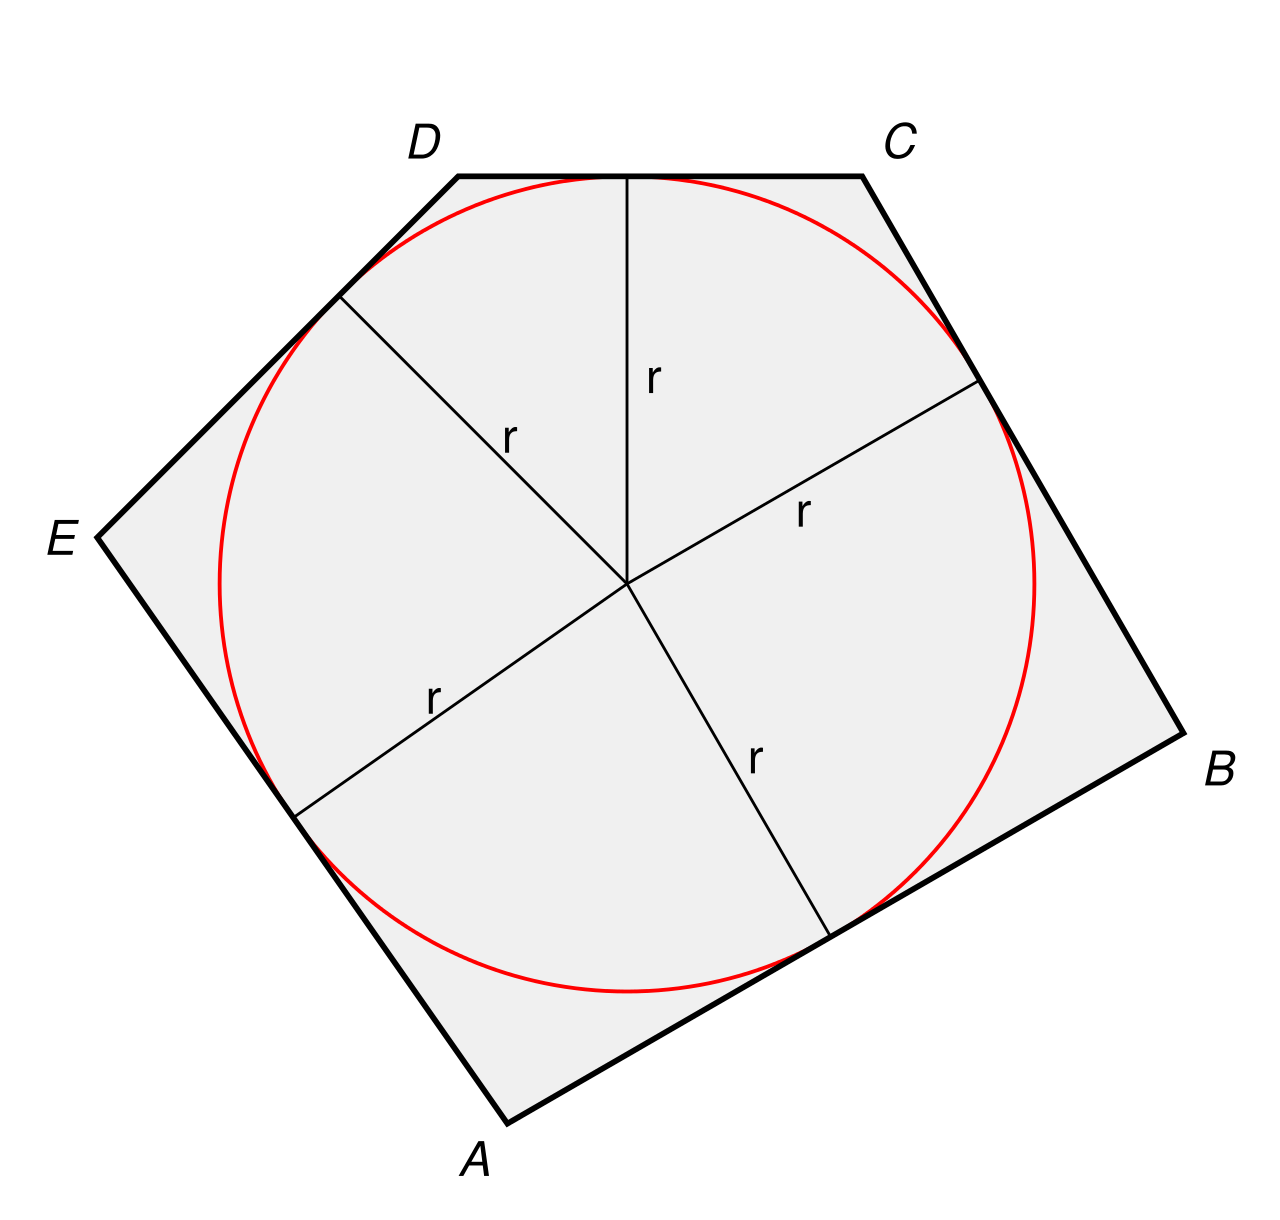
\includegraphics[width=6cm]{Pentagon-inscribed-circle.svg.png}
			\caption{Darstellung eines Inkreis \cite{b1}}
			\label{inkreis}
		\end{center}
	\end{figure}
	
	\section{Idee 1:}
	\subsection{Mittelpunkt des Inkreis}
	Um die Mittelpunkt eines Polygon zu Berechnen wird der durchschnitt aller Eckpunkte berechnet.
	Die Komplexität zum Berechnen des Mittelpunkt des Inkreis beträgt $\mathcal{O}(n)$. 
	\subsection{Radius des Inkreis}
	Sobald der Mittelpunkt des Inkreises bekannt ist muss man nur noch den Radius berechnen. Dieser soll Maximal sein aber nicht über eine Kante des Polygons gehen. Hierfür berechnet man alle Distanzen zu allen Kanten des Polygons. Die kürzeste Distanz ist der Radius des Inkreis.\\
	Zu Berechnung der Distanz vom Mittelpunkt zu einer Kante des Polygons wird die Flächenformel des Dreiecks $A = \frac{1}{2}*b*h$ zu $h=\frac{2*A}{b}$ umgestellt. 
	Alles zusammen gesetzt ergibt die Formel zu Berechnung des Abstands von Punkt $P_0$ zur Strecke $P_1P_2$:
	\[ d(P_0,P_1,P_2) = \frac{|(x_2-x_1)(y_1-y_0) - (x_1-x_0)(y_2-y_1)|}{\sqrt{(x_2-x_1)^2+(y_2-y_1)^2}} \]
	\subsection{Fazit}
	Die Komplexität zum Berechnen des Radius des Inkreis beträgt $\mathcal{O}(n)$.\\
	Leider führt diese Idee nicht immer zu richtigen Lösung. In der Abbildung \ref{fail} ist einer dieser Fälle dargestellt.\\
	\begin{figure}[h]
		\begin{center}
			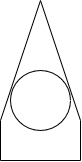
\includegraphics[width=3cm]{CircleFail.png}
			\caption{Problem des Verfahrens}
			\label{fail}
		\end{center}
	\end{figure}
	Um das Problem zu lösen müssten mehrere Mittelpunkte getestet werden. Hierfür müsste man den voraussichtlich den Druchschnittspunkt aller Eckpunktkombinationen testen. Dies wären in einem naiven Ansatz $n!$ verschiedene Kombinationen. Da aber ein Durchschnitt mit drei Punkten erst sinn macht könnte man den Aufwand etwa reduzieren. Es bleibt aber trotzdem noch bei einem großen aufwand. Die Technik macht nur Sinn bei einem regulärem Polygon.
	
	\section{Lineare Programmierung}
	Es ist möglich die Lösung mithilfe der Linearen Optimierung zu lösen. So gibt es eine Matrix $A \in \mathbb{R}^{m,n}$, ein Vektor $\vec{b} \in \mathbb{R}^{m,1}$ und ein Vektor $\vec{c} \in \mathbb{R}^{1,n}$.\\
	Es wird ein zulässiger Lösungsvektor $\vec{x} \in \mathbb{R}^{n}$ gesucht der
	\[ \vec{c}\vec{x} = c_1x_1 + c_2x_2+ ... + c_nx_n \]
	maximiert.
	Das Optimierungsproblem kann so dargestellt werden:
	\[ \text{max}\{\vec{c}\vec{x} | A\vec{x} \leq b, \vec{x} \geq 0\} \]
	\cite{b2}\\
	Unser Vektor $\vec{x}$ enthält den Mittelpunkt und Radius des Inkreises:
	\[ \vec{x} = \left(\begin{array}{c}x\\y\\r\end{array}\right) \]
	Die Basiszielfunktion ist:
	\[\max \vec{c}\vec{x} = c_1*x+c_2*y+c_3*r \]
	Da wir aber nicht die Koordinaten maximieren wollen sondern nur den Radius können wir die Zielfunktion stark vereinfachen:
	\[ \max \vec{c}\vec{x} = 0*x+0*y+1*r = r \]
	\textit{linprog} findet nun das Minimum. Deshalb muss die Zielfunktion muss noch negiert werden weil das Maximum benötigt wird.\\
	\[ \min \vec{c}\vec{x} = 0*x+0*y-1*r = -r \]
	Der Ergebnisraum wird durch die Nebenbedingungen beschränkt, die jeweils durch die Kanten des Polygons definiert werden. So darf der Abstand zwischen dem Zentrum und der Kante nicht größer als der Radius sein. Bei n Kanten gibt es die n Nebenbedingungen. Für die Kante $g_n$ entsteht die Ungleichung:
	\[  r \leq d(\left(\begin{array}{c}x\\y\end{array}\right), g_n) \]
	\[  r \leq n_1 * x + n_2 * y - b \]
	\[  b \geq -n_1 * x - n_2 * y + r \]
	$\vec{n}$ entzieht man der Hessesche Normalenform:
	\[ \vec{n} =  \left(\begin{array}{c}n_1\\n_2\end{array}\right) = \left(\begin{array}{c}\frac{p_y}{\sqrt{p_x^2+p_y^2}}\\\frac{-p_x}{\sqrt{p_x^2+p_y^2}}\end{array}\right) \]
	$p_x$ und $p_x$ ist der Vektor einer Kante $g_n$:\\
	\[ \vec{p} =  \left(\begin{array}{c}p_x\\p_y\end{array}\right) = \left(\begin{array}{c}x_{n+1} - x_n\\y_{n+1} - y_n\end{array}\right) \]
	Zum Lösen dieses Problems wird die Bibliotheksmethode \textit{linprog} aus matlab verwendet.\\
	\\
	\textbf{Beispiel für ein einfaches Quadrat:}\\
	Das Quadrat ist definiert mit den Punkten:
	\[\left(\begin{array}{c}0\\0\end{array}\right) , \left(\begin{array}{c}10\\0\end{array}\right),\left(\begin{array}{c}10\\10\end{array}\right),\left(\begin{array}{c}0\\10\end{array}\right)\]
	Das Matrix $A$ und der Vektor $b$ sieht so aus:
	\[A = \begin{pmatrix}
		0 & -1 & 1 \\
		1 & 0 & 1 \\
		0 & 1 & 1 \\
		-1 & 0 & 1 \\
	\end{pmatrix}\]
	\[b = \begin{pmatrix}
		0 \\
		10\\
		10\\
		0\\
	\end{pmatrix}\]
	Die resultierenden Nebenbedingungen sind:
	\[ -c_2*y+r \leq 0 \]
	\[ c_1*x+r \leq -10 \]
	\[ c_2*y+r \leq -10 \]
	\[ -c_1*x+r \leq 0 \]
	 Das Ergebnis einspricht: $x = 5, y = 5, r = -5$.\\
	 Der Radius muss immer Positiv sein dementsprechend nimmt man immer den Betrag des Radius.\\
	\textbf{Beispiel für ein größeres Polygon:}\\
	Das Ergebnis für das größere Polygon einspricht:\\
	 $x = 472.57, y = 476.66, r = 438.59$.\\
	Durch einen Plot scheint das Ergebnis zu stimmen.
	\begin{figure}[h]
		\begin{center}
			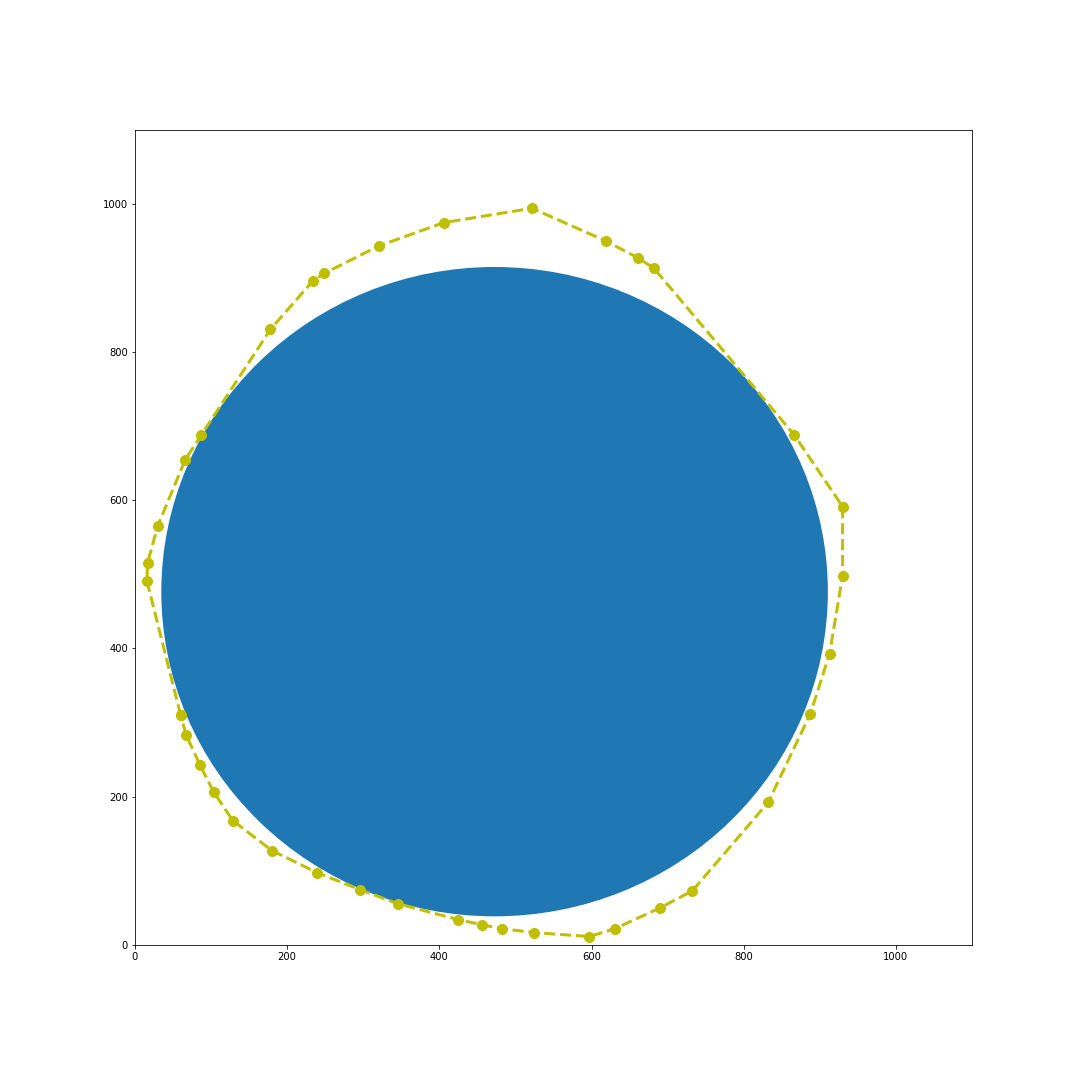
\includegraphics[width=8cm]{Inscribed.png}
			\caption{Der größte Inkreis für ein größeres Polygon}
			\label{fail}
		\end{center}
	\end{figure}

	
	\begin{thebibliography}{00}
		\bibitem{b1}https://de.wikipedia.org/wiki/Inkreis\#/media/Datei:Pentagon-inscribed-circle.svg
		\bibitem{b2}https://de.wikipedia.org/wiki/Lineare\_Optimierung
	\end{thebibliography}
	
	
	
	\section{Anhang}
	Berechnung des Mittelpunkts des Polygons aus Idee 1
	\begin{lstlisting}[basicstyle=\tiny]
	public Point getMiddle(){
		final double avgX = cords.stream().mapToDouble(p-> p.getX()).sum()/(cords.size()-1);
		final double avgY = cords.stream().mapToDouble(p-> p.getY()).sum()/(cords.size()-1);
		return new Point(avgX, avgY);
	}
	\end{lstlisting}
	Berechnung des Inkreis des Polygons aus Idee 1
	\begin{lstlisting}[basicstyle=\tiny]
	public Circle getLargestInscribedCircle(){
		final Point middle = getMiddle();
		
		double minDistance = Double.POSITIVE_INFINITY;
		for(int counter = 1; counter < cords.size() ; counter++){
			final Segment edge = new Segment(cords.get(counter-1), cords.get(counter));
			final double distance = edge.distanceToPoint(middle);
			if(distance < minDistance)
			minDistance = distance;
		}
		
		return new Circle(middle, minDistance);
	}
	\end{lstlisting} 
	\lstset{language=Matlab,
		showspaces=false,
		showtabs=false,
		breaklines=true,
		tabsize=2,
		showstringspaces=false,
		breakatwhitespace=true,
		commentstyle=\color{pgreen},
		keywordstyle=\color{pblue},
		stringstyle=\color{pred},
		basicstyle=\ttfamily
	}
 	Berechnung des Inkreis des Polygons mit Matlab und LP
\begin{lstlisting}[basicstyle=\tiny]
data = [[0 0] ,[10 0], [10 10], [0 10], [0 0]];
len = length(data)
data = transpose(reshape(data, 2, len/2));
len = length(data)

A = zeros(len-1,3);
b = zeros(len-1,1);
for i=1:len-1
	first = data(i,:);
	second = data(i+1,:);
	
	px = second(1)-first(1);
	py = second(2)-first(2);
	
	n1 = py / sqrt(px^y + py^2);
	n2 = -px / sqrt(py^2 + py^2);
	A(i,:) = [-n1,-n2,1];
	b(i) = -(n1*first(1)+n2*first(2));
end

disp(A)
disp(b)
X = linprog([0 0 -1],A,b);
disp(X)
\end{lstlisting}  



\end{document}
